%%%%%%%%%%%%%%%%%%%%%%%%%%%%%%%%%%%%%%%%%%%%%%%%%%%%%%%%%%%%%%%%%%%%%%%%%%%%%%%
%
% 02 - Requerimientos
%
%%%%%%%%%%%%%%%%%%%%%%%%%%%%%%%%%%%%%%%%%%%%%%%%%%%%%%%%%%%%%%%%%%%%%%%%%%%%%%%

\chapter{\textcolor{azulescom}{Requerimientos}}

\section{Requisitos del sistema}

Para que \textit{SkyPrice} funcione correctamente, es necesario que el sistema
cumpla con los requerimientos mínimos de hardware y software que se detallan a
continuación. En el cuadro \ref{tab:requerimientos-desktop} se presentan los
requerimientos mínimos y recomendados para la versión de escritorio de \textit{SkyPrice}.
En el cuadro \ref{tab:requerimientos-movil} se presentan los requerimientos mínimos
y recomendados para la versión móvil de \textit{SkyPrice}.

% Tabla de requerimientos para la versión de escritorio
\begin{table}[H]
\centering
\begin{tabular}{|p{4cm}|p{4cm}|p{4cm}|}
\hline
\textbf{Componente} & \textbf{Mínimo} & \textbf{Recomendado} \\ \hline
Procesador & 1 GHz & 2 GHz \\ \hline
Memoria RAM & 1 GB & 2 GB \\ \hline
Pantalla & 1024x768 & 1280x1024 \\ \hline
Conexión a internet & 1 Mbps & 10 Mbps \\ \hline
Navegadores & Chrome 30, Firefox 35, IE 11, Safari 8 & Chrome 40, Firefox 40, IE 11, Safari 8 \\ \hline
\end{tabular}
\caption{Requerimientos para la versión de escritorio}
\label{tab:requerimientos-desktop}
\end{table}

% Tabla de requerimientos para la versión móvil
\begin{table}[H]
\centering
\begin{tabular}{|p{4cm}|p{4cm}|p{4cm}|}
\hline
\textbf{Componente} & \textbf{Mínimo} & \textbf{Recomendado} \\ \hline
Procesador & 1 GHz & 2 GHz \\ \hline
Memoria RAM & 1 GB & 2 GB \\ \hline
Pantalla & 480x800 & 720x1280 \\ \hline
Conexión a internet & 3G/HSPA+ (1.5 Mbps) & 4G/LTE (10 Mbps) \\ \hline
Navegadores & Chrome 30, Firefox 35, IE 11, Safari 8 & Chrome 40, Firefox 40, IE 11, Safari 8 \\ \hline
\end{tabular}
\caption{Requerimientos para la versión móvil}
\label{tab:requerimientos-movil}
\end{table}

\section{Compatibilidad de navegadores}

\textit{SkyPrice} ha sido probado en los siguientes navegadores web:

\begin{itemize}
\item \textbf{Google Chrome 40}
\item Mozilla Firefox 35
\item Internet Explorer 11
\item Safari 8
\end{itemize}

Se recomienda utilizar Google Chrome 40 para una mejor experiencia de usuario.

\section{Acceso a la aplicación}
La aplicación web de \textit{SkyPrice} está disponible en la siguiente dirección:

\begin{center}
\url{https://skyprice.xyz}
\end{center}

En la figura \ref{fig:skyprice-xyz-qr} se muestra un código QR que puede ser escaneado
para acceder a la aplicación.

% Imagen con el código QR de skyprice.xyz
\begin{figure}[H]
  \centering
  
\includegraphics[width=0.3\textwidth]{imagenes/02-requerimientos/skyprice-xyz-qr.png}
  \caption{Código QR de skyprice.xyz}
  \label{fig:skyprice-xyz-qr}
\end{figure}

Una vez que el usuario accede a la aplicación, se mostrará la página de inicio de \textit{SkyPrice},
donde podrá encontrar directamente el formulario de estimación de precios de mercado para departamentos.
En la figura \ref{fig:skyprice-home} se muestra la página de inicio de \textit{SkyPrice}
en la versión de escritorio.

% Imagen de la página de inicio de skyprice.xyz
\begin{figure}[H]
  \centering
  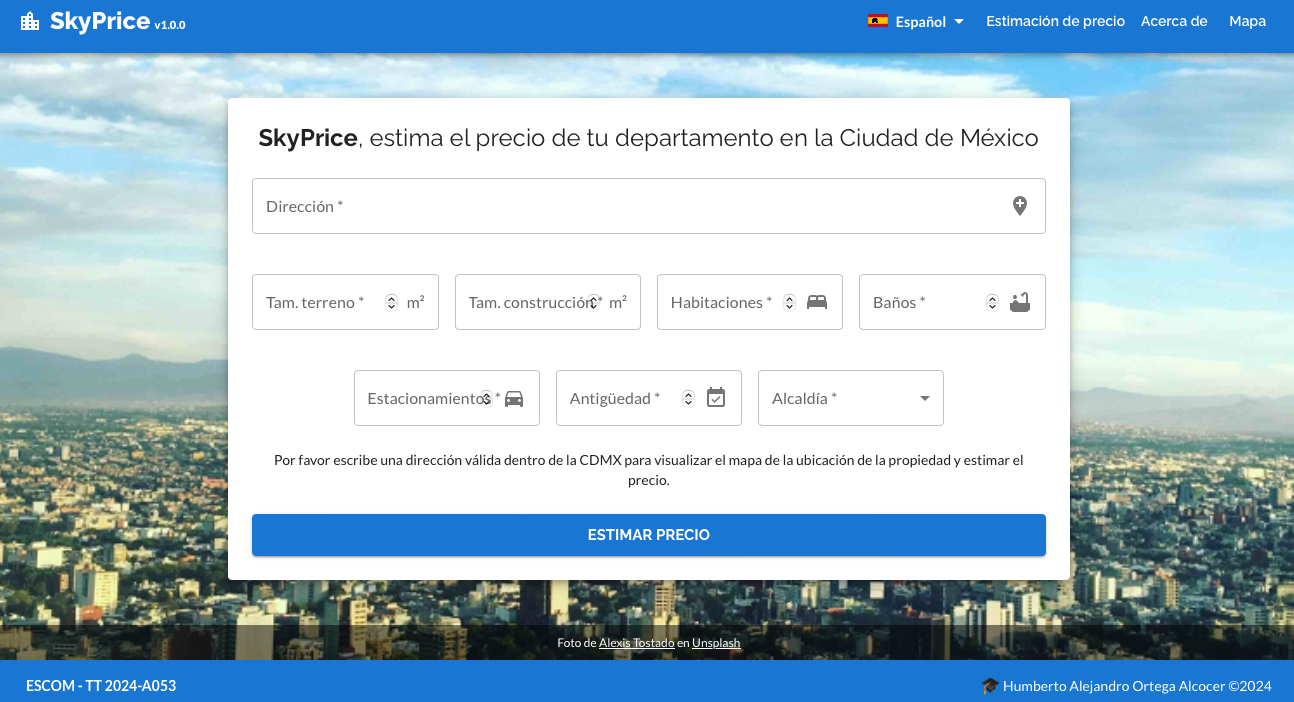
\includegraphics[width=1.0\textwidth]{imagenes/02-requerimientos/skyprice-home.png}
  \caption{Página de inicio de SkyPrice}
  \label{fig:skyprice-home}
\end{figure}

\section{Navegación}
Para  navegar en la aplicación, los usuarios pueden utilizar la barra de navegación
ubicada en la parte superior de la página. En la barra de navegación se encuentran
los siguientes elementos:

\begin{itemize}
\item \textbf{Logo de SkyPrice}: Al hacer clic en el logo de SkyPrice, el usuario será
redirigido a la página de inicio de la aplicación.
\item \textbf{Selección de idioma}: Los usuarios pueden seleccionar el idioma de la aplicación
desde la barra de navegación. Los idiomas disponibles son: español, inglés, francés y portugués.
\item \textbf{Estimación de precio}: Al hacer clic en el enlace ``Estimar precio'', el usuario
será redirigido al formulario de estimación de precios de mercado para departamentos, que se
encuentra en la página de inicio.
\item \textbf{Acerca de}: Al hacer clic en el enlace ``Acerca de'', el usuario será redirigido
a la página de información sobre el proyecto SkyPrice.
\item \textbf{Mapa}: Al hacer clic en el enlace ``Mapa'', el usuario será redirigido a la página
del mapa interactivo con los anuncios de departamentos en la Ciudad de México y
los conjuntos de datos disponibles.
\end{itemize}

En la figura \ref{fig:barra-navegacion} se muestra un ejemplo de la barra de navegación
de \textit{SkyPrice}.

% Imagen de la barra de navegación de SkyPrice
\begin{figure}[H]
  \centering
  
\includegraphics[width=1.0\textwidth]{imagenes/02-requerimientos/barra-navegacion.png}
  \caption{Barra de navegación de SkyPrice}
  \label{fig:barra-navegacion}
\end{figure}

